%
%  Thesis main document
%
%  Created by Mathias Dalheimer on 2007-02-14
%  Copyright (c) 2007. All rights reserved.
%
\documentclass[11pt]{article}

% Use utf-8 encoding for foreign characters
\usepackage[utf8]{inputenc}

% Setup for fullpage use
\usepackage{fullpage}
\usepackage{url}
%\usepackage{german}

% Uncomment some of the following if you use the features
%
% Running Headers and footers
%\usepackage{fancyhdr}
%\pagestyle{fancy} % options: empty , plain , fancy
%\renewcommand{\headrulewidth}{1pt} % customise the layout...
%\lhead{}\chead{}\rhead{}
%\lfoot{}\cfoot{\thepage}\rfoot{}

%\fancyhead[LE,RO]{\slshape \rightmark} 
%\fancyhead[LO,RE]{\slshape \leftmark} 
%\fancyfoot[LE, RO]{\thepage} 

%%% SECTION TITLE APPEARANCE
\usepackage{sectsty}
\allsectionsfont{\sffamily\mdseries\upshape} % (See the fntguide.pdf for font help)
% (This matches ConTeXt defaults)

\setlength{\parindent}{0cm}
\clubpenalty=1500
\widowpenalty=2000

\usepackage{ngerman}

% Multipart figures
%\usepackage{subfigure}
%\usepackage{lib/algorithm2e}

% More symbols
\usepackage{amsmath}
%\usepackage{amssymb}
\usepackage{latexsym}

% Surround parts of graphics with box
%\usepackage{boxedminipage}

% Package for including code in the document
%\usepackage{listings}

% If you want to generate a toc for each chapter (use with book)
%\usepackage{minitoc}

% This is now the recommended way for checking for PDFLaTeX:
\usepackage{ifpdf}

%\newif\ifpdf
%\ifx\pdfoutput\undefined
%\pdffalse % we are not running PDFLaTeX
%\else
%\pdfoutput=1 % we are running PDFLaTeX
%\pdftrue
%\fi

\ifpdf
\usepackage[pdftex]{graphicx}
\else
\usepackage{graphicx}
\fi


\usepackage{listings}  
\lstset{numbers=left, numberstyle=\tiny,numbersep=5pt}  
\lstset{language=Xml, basicstyle=\small, frame=shadowbox}  

\usepackage[hypertexnames=false,pdftex]{hyperref}
\hypersetup{
pdfauthor = {Mathias Dalheimer},
pdftitle = {Designing Message-oriented Applications with MQS and
SEDA}
pdfsubject = {},
pdfkeywords = {Grid Computing}
pdfcreator = {LaTeX with hyperref package},
pdfproducer = {dvips + ps2pdf}}
\usepackage{algorithmic}
\usepackage{algorithm}
\renewcommand{\algorithmicrequire}{\textbf{Input:}} 
\renewcommand{\algorithmicensure}{\textbf{Output:}}

%%%%%%%%%%%%%%%%%%%%%%%%%%%%%%%%%%%%%%%%%%%%%%%%%%%%%%%%%%%%%%%%%%%%
\newcommand{\outcome}[1]{\mathtt{#1}}
\newcommand{\jobpredicate}[1]{\mathtt{#1}}

\newcommand{\stateset}{\mathcal{S}}
\newcommand{\actionset}{\mathcal{A}}
\newcommand{\transprob}{\mathcal{P}}
\newcommand{\reward}{\mathcal{R}}
\newcommand{\return}{\mathit{R}}
\newcommand{\policy}{\pi}
\newcommand{\plainstatevaluefunct}[1]{V^{#1}}
\newcommand{\statevaluefunct}{\plainstatevaluefunct{\policy}}
\newcommand{\optstatevaluefunct}{\plainstatevaluefunct{*}}
\newcommand{\actionvaluefunct}{Q^\policy}
\newcommand{\optactionvaluefunct}{Q^*}
%%%%%%%%%%%%%%%%%%%%%%%%%%%%%%%%%%%%%%%%%%%%%%%%%%%%%%%%%%%%%%%%%%%%
\newcommand{\PG}{PHASTGrid\ }
\newcommand{\SM}{Storagemanager\ }

\title{\textsf{Designing Message-oriented Applications with libmqs and
libseda}}
\author{ Mathias Dalheimer\\
\url{dalheimer@itwm.fhg.de}}

\date{Version 0.1, \today\\
}

\begin{document}

\ifpdf
\DeclareGraphicsExtensions{.pdf, .jpg, .tif}
\else
\DeclareGraphicsExtensions{.eps, .jpg}
\fi

\maketitle


\tableofcontents

\section{Introduction}\label{sec:introduction}
Building blocks of message-oriented applications are message brokers.
Clients connect to message brokers and exchange messages adressed to
logocal URIs instead of communicating directly with each other. In order
to support the development of message-oriented applications, the libmqs
and libseda libraries have been written.

\section{Anatomy of an Application}\label{sec:anatomy of an application}
As a quick introduction, I will present some of the functionality of the
libraries in this section. I assume you're familiar with the SEDA
architectural approach. Basically, applications process incoming
messages in stages. Each stage contains a threadpool. Stages are
separated with queues. The work to be done is put in the inqueue of a
stage. A thread dequeues it and applies a strategy to it. Depending on
the strategy one or several messages are issued to the environment -
which means that other stages might pick them up. Decorators provide
another way of adding behaviour to a stage: Think of them as a FIFO pipe
that all messages must pass before they are processed.

The libmqs provides abstractions for connecting to a message broker,
sending and receiving messages etc.
\begin{figure}[htbp]
  \begin{center}
    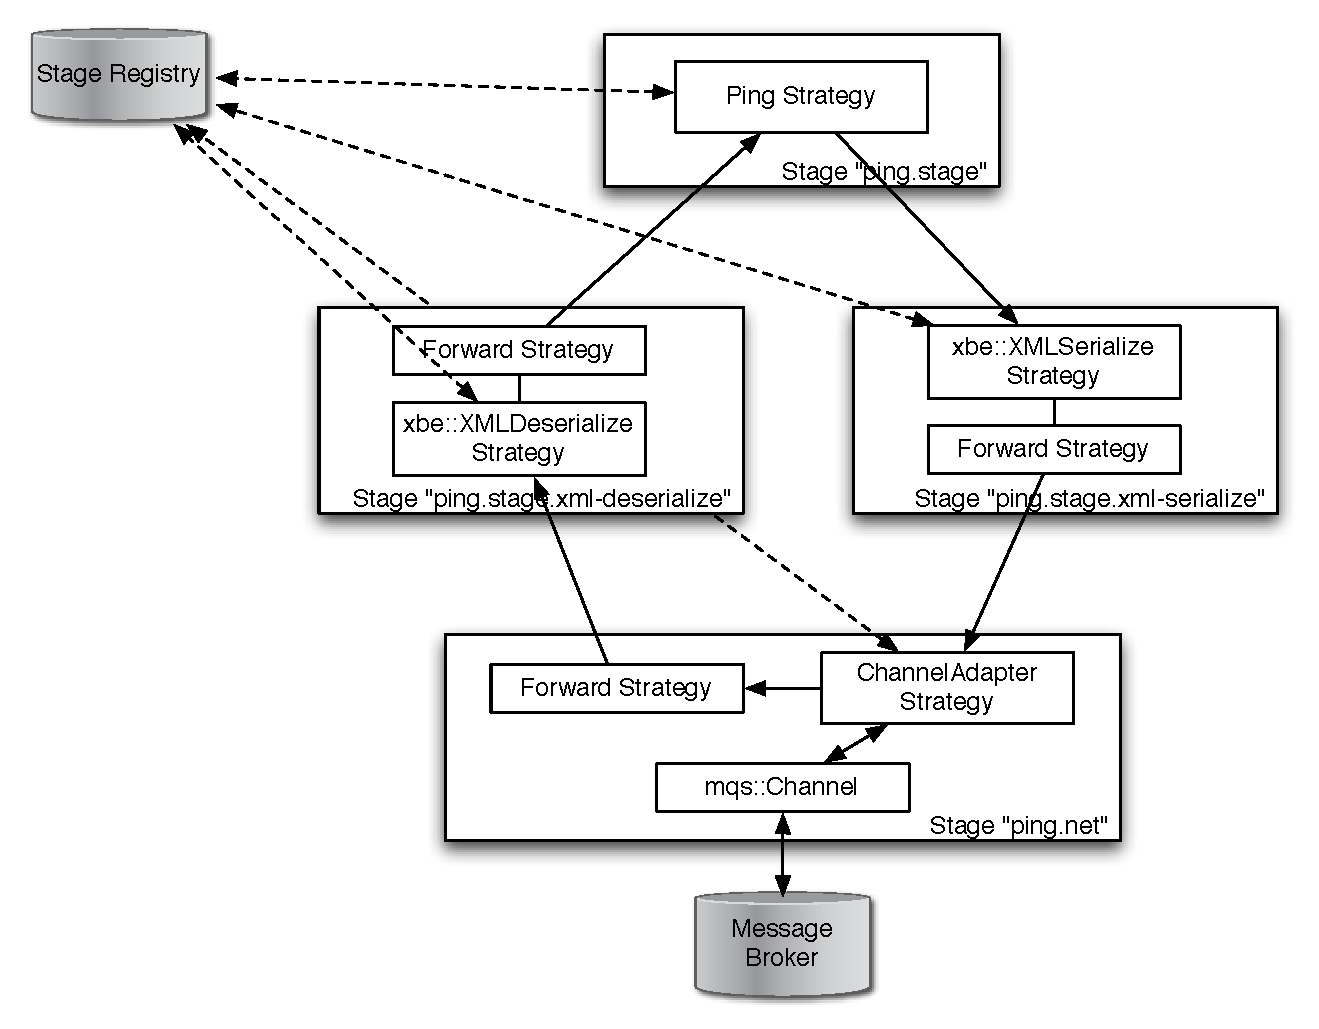
\includegraphics[width=12cm]{MQS-SEDA-Architecture.pdf}
    \caption{The building blocks of the Pingpong architecture. Only
    the Ping part is shown.}
    \label{fig:mqs-seda-architecture}
  \end{center}
\end{figure}

The easiest way to understand this is to look at some application. I
use the famous PingPong example where two application send each other
"`ping"' and "`pong"' messages. You can find the corresponding source
code in \verb|xbe/tests/xbe/PingPongTest.cpp|. 

The structure of the application is shown in figure
\ref{fig:mqs-seda-architecture}. The connection to the Message Broker is
made in the "`ping.net"' stage. An mqs Channel object receives the
messages and puts them in the ChannelAdapter Strategy inqueue. They are
then forwarded to the xml-deserialize stage, where an XML encoding is
removed. Again, the messages are forwarded to the "`ping.stage"' where a
Ping Strategy implements the behaviour of the application - i.e., it
responds with a "`pong"' message for each incoming "`ping"' message.
Outgoing messages are serialized and forwarded to the ChannelAdapter
strategy, which sends them over the mqs Channel to the Message Broker.

The connection between the different stages is made through the Stage
Registry. At startup, all stages register themselves with a unique
identifier at the registry. The ForwardStrategies (and the PingStrategy)
are initialized with the identifier of the Strategy they should sent
their messages to. This way, it is easy to link together new functions
and to introduce new stages.

\end{document}
